\chapter{VLANs and Subnetting}

\thispagestyle{standard}
\pagestyle{standard}

The given network was 192.168.1.0/24, which had to be divided into 4 subnets. Each subnet corresponded to a specific \ac{VLAN}.

\begin{table}[h]
\centering
\begin{tabular}{r||r|r|r|r|}
\textbf{VLAN} & \textbf{Hosts} & \textbf{Network ID/Subnet} & \textbf{First usable IP} & \textbf{Broadcast IP} \\

		\hline
10 & 120 & 192.168.1.0/25 & 192.168.1.1 & 192.168.1.127  \\
20 & 60 & 192.168.1.128/26 & 192.168.1.129 & 192.168.1.191  \\
30 & 30 & 192.168.1.192/27 & 192.168.1.193 & 192.168.1.223  \\
99 & 10 & 192.168.1.224/28 & 192.168.1.224 & 192.168.1.239  \\

\end{tabular}
\caption{VLANs and Subnets}
\label{tab:vlan_subnets}
\end{table}

The final subnets that were used in the lab can be seen in table  \ref{tab:vlan_subnets}.

The first usable IP address in each subnet was assigned to the subinterface of that network at the router.

\chapter{Topology}

The following topology (figure \ref{img:topo}, taken from the moodle instructions) had to be recreated in the lab.

\begin{figure}[H]
	\centering
	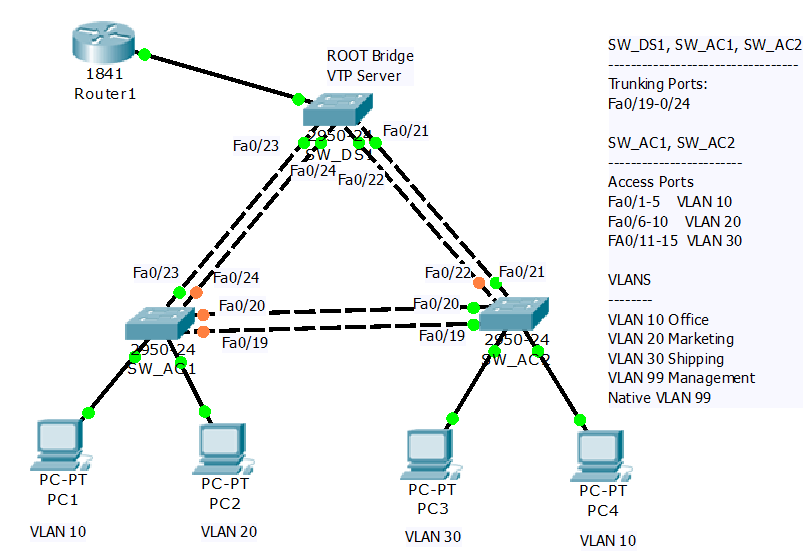
\includegraphics[width=0.9\textwidth]{img/topo.png}
	\caption{Topology (Moodle)}
	\label{img:topo}
\end{figure}

\section{Basic configuration}

Each device was configured with basic settings like hostname, \ac{MOTD}, a secret enable password, disabled IP domain lookup, synchronous logging on line console 0 and the service password-encryption, which prevents passwords from being displayed in cleartext in the start-up and running configuration.

\lstset{escapeinside={\%*}{*)},numbers=left}%oder numbers=left
\begin{lstlisting}[caption={Basic configuration},label={lst:debug_s3},language={}]
enable
conf terminal
hostname SW_AC1
banner motd # Unauthorized access prohibited! #
enable secret cisco
service password-encryption
no ip domain-lookup
line con 0
	synchronous logging
\end{lstlisting}

These settings were applied to every device, with a respectively different hostname.

\section{Spanning Tree}

The use of the \ac{STP} allows to detect loops in the network and creates a first redundancy layer. \ac{STP} uses a tree structure in which every switch (bridge) in the network knows the best path to the root bridge. Redundant paths to the root bridge will be blocked for normal traffic.

\texttt{SW\_DS1} had to be configured as root bridge.

\lstset{escapeinside={\%*}{*)},numbers=left}%oder numbers=left
\begin{lstlisting}[caption={\ac{STP} configuration root},label={lst:stp},language={}]
conf terminal
spanning-tree mode pvst
spanning-tree vlan 1,10,20,30,99 priority 4096
\end{lstlisting}

This is the configuration for the root bridge. The bridge with the lowest bridge ID will become root bridge. In this configuration the ID is \texttt{4096}. The other switches in the network have been left at the default priority which is higher and enables \texttt{SW\_DS1} to become root.

The \ac{PVST} mode has been used to spawn a \ac{STP} instance per VLAN. This would allow load balancing of certain \acp{VLAN} to different paths, but this was not used in this lab. The \ac{PVST} mode was used for all configured \ac{VLAN}s.

\chapter{VTP}

The \ac{VTP} allows the distribution of configured \ac{VLAN}s to all switches in the VTP domain. This allows easier reconfiguration of VLANs. For VTP to work one switch has to act as the VTP server and the switches that need to receive the configuration have to be set as VTP clients.

Similar to the STP root bridge, \texttt{SW\_DS1} had to be configured to act as \ac{VTP} server.

\lstset{escapeinside={\%*}{*)},numbers=left}%oder numbers=left
\begin{lstlisting}[caption={\ac{VTP} and VLAN},label={lst:vtps},language={}]
vlan 10 name Office
vlan 20 name Marketing
vlan 30 name Shipping
vlan 99 name Management

vtp mode server
vtp version 2
vtp domain lab
vtp password cisco
\end{lstlisting}

The commands listed above create the 4 \acp{VLAN} and the \ac{VTP} server on \texttt{SW\_DS1}.

Version 2 had to be used, as we encountered the following problem when using VTP V3:

VTP V3 rejected the deletion of \acp{VLAN} on the VTP server as well as on the VTP clients. The following error message appeared when trying to delete VLANs: \\
\textit{VTP VLAN configuration not allowed when device is not the primary server for vlan database.}

Moreover important was to explicitly set a VTP password, otherwise the following message may appear: \\
\textit{*** MD5 digest checksum mismatch on trunk: Fa0/xx ***}

The client configuration for the switches can be seen in listing \ref{lst:vtps}.

\lstset{escapeinside={\%*}{*)},numbers=left}%oder numbers=left
\begin{lstlisting}[caption={\ac{VTP} client},label={lst:vtps},language={}]
vtp mode client
vtp version 2
vtp domain lab
vtp password cisco
\end{lstlisting}

\chapter{\ac{VLAN} setup}

In this chapter, the ports on the switch had to be configured as either VLAN access ports, or trunk ports for the uplinks to the other switches.

The port VLAN assignment can be seen in table \ref{tab:vlan_ports}.

\begin{table}[h]
\centering
\begin{tabular}{r||r}
\textbf{Ports} & \textbf{VLANs}  \\

		\hline
Fa0/1-5 & 10 \\
Fa0/6-10 & 20 \\
Fa0/11-15 & 30    \\
Fa0/19-24 & Trunk ports  \\
everything else & 1

\end{tabular}
\caption{VLANs to ports}
\label{tab:vlan_ports}
\end{table}

\lstset{escapeinside={\%*}{*)},numbers=left}%oder numbers=left
\begin{lstlisting}[caption={Access port configuration},label={lst:accport},language={}]
int range fa0/1 - 5
switchport mode access
switchport access vlan 10
\end{lstlisting}

\lstset{escapeinside={\%*}{*)},numbers=left}%oder numbers=left
\begin{lstlisting}[caption={Trunk port configuration},label={lst:accport},language={}]
int fa0/21
switchport mode trunk
switchport trunk allowed vlan 10,20,30,99
switchport trunk native vlan 99
\end{lstlisting}

The commands in listing \ref{lst:accport} have been adapted to match the different VLANs.
The access ports have been configured on both \texttt{SW\_AC1} and \texttt{SW\_AC2}.

The native VLAN is 99, which is also the management VLAN. From a security point of view it's not recommended to set the native VLAN to the same as the management VLAN. \\ 
The native VLAN will not be tagged (802.1Q) when transmitted through the trunk port. For ease of configuration some unused ports where assigned to the Management VLAN.

To test this configuration we put a PC in each VLAN on each switch and used the `ping' tool for verification, which showed a successful configuration.

% ausgabe einf�gen?

\chapter{Inter-VLAN Routing}

To make communication between the VLANs possible a router needs to be used. This type of setup is normally known as router on a stick. Subinterfaces with IP addresses for each subnets (see table \ref{tab:vlan_subnets}) have been configured. Thus all PCs are able to communicate with the router and also with PCs on different subnets (when the default gateway on the PCs is correctly set to the IP address of the subinterface on the router).

\lstset{escapeinside={\%*}{*)},numbers=left}%oder numbers=left
\begin{lstlisting}[caption={Router configuration},label={lst:routervlan},language={}]
conf terminal
int gig0/0.10
encapsulation dot1q 10
ip address 192.168.1.1 255.255.255.128
\end{lstlisting}

The commands in listing \ref{lst:routervlan} will create a subinterface on gig0/1 and set the encapsulation to the IEEE 802.1Q standard. Then an IP address is assigned to that interface. This commands have been adopted for every subinterface.

For the native VLAN, the encapsulation line had been changed to:

\texttt{encapsulation dot1Q 99 native}

to mark VLAN 99 as the native VLAN.

\chapter{Remote Administration}

In this chapter remote access via \ac{SSH} had to be configured for each switch and the router.

The management interface on the switches was created in the management \ac{VLAN}.

\lstset{escapeinside={\%*}{*)},numbers=left}%oder numbers=left
\begin{lstlisting}[caption={Management interface},label={lst:sw99},language={}]
conf terminal
interface Vlan99
 ip address 192.168.1.226 255.255.255.240
 no shutdown
\end{lstlisting}

The IP addresses were assigned beginning with \texttt{192.168.1.225} for the router and ending with \texttt{192.168.228} for \texttt{SW\_AC2}.

\section{SSH}

\ac{SSH}(v2) is a protocol for a secure connection to another device which should be used instead of insecure protocols like telnet.
For \ac{SSH} access a domain name, a user and certificates have to be created.

\lstset{escapeinside={\%*}{*)},numbers=left}%oder numbers=left
\begin{lstlisting}[caption={SSH and user creation},label={lst:ssh},language={}]
conf terminal
ip domain-name its.its
crypto key generate rsa 1024
username admin secret cisco
line vty 0 4
login local
transport input ssh
\end{lstlisting}

The commands from listing \ref{lst:ssh} will configure SSH on the device. The key length has been set to 1024 bit for convenience, as it would take more time to create a key with a length of 2048 bit. Moreover, the virtual terminal line has been configured to only allow ssh input and use the local database for authentication.

\chapter{Layer 2 Security}

In this chapter Layer 2 security was applied to the switches.

First, unused switchports were shut down, as seen in listing \ref{lst:unused}.

\lstset{escapeinside={\%*}{*)},numbers=left}%oder numbers=left
\begin{lstlisting}[caption={Shutdown unused ports},label={lst:unused},language={}]
conf terminal
ip range fa0/3 - 20
shutdown
\end{lstlisting}

This command has been adopted to all switches, the example was applied to \texttt{SW\_DS1}.

Another security feature was to allow only a certain amount of \ac{MAC} addresses per switchport and deactivate the port if more addresses are seen.

\lstset{escapeinside={\%*}{*)},numbers=left}%oder numbers=left
\begin{lstlisting}[caption={Sticky MAC addresses},label={lst:mac},language={}]
conf terminal
ip range fa0/11 - 15
 switchport port-security
 switchport port-security mac-address sticky 1
 switchport port-security violation shutdown
\end{lstlisting}

Listing \ref{lst:mac} shows such a configuration. The maximum allowed \ac{MAC} addresses is set to 1, which means that only one device is allowed on that port. If a second device with a different \ac{MAC} address connects to the port a violation will be thrown and the port will shut down. In order to reactivate the port it has to be manually shut down and enabled again.

\chapter{DHCP}

\ac{DHCP} is a method to distribute IP addresses (in form of DHCP leases) in a network automatically. Almost all operating systems have available \ac{DHCP} clients.

The router was configured to act as \ac{DHCP} server, distributing IP addresses to clients in the \ac{VLAN}s.

\lstset{escapeinside={\%*}{*)},numbers=left}%oder numbers=left
\begin{lstlisting}[caption={DHCP},label={lst:dhcp},language={}]
ip dhcp pool VLAN10
 network 192.168.1.0 255.255.255.128
 domain-name VLAN10
 default-router 192.168.1.1
\end{lstlisting}

With these commands (\ref{lst:dhcp}) the router will act as a \ac{DHCP} server and will distribute IP addresses in the \texttt{192.168.1.0/25} subnet. Those commands were also set for the other VLANs.

\section{DHCP Snooping}

DHCP Snooping is a method to block rogue DHCP server which can handle out wrong IP addresses. It can also be used to limit the amount of IP addresses a port can request in a given amount of time in order to counterfeit IP address shortage. DHCP responses may also be restricted to certain ports. In example an access port, where a client computer is connected, should nit issue DHCP responses. As DHCP has no authentication mechanism DHCP snooping should be implemented if security is from importance.

\lstset{escapeinside={\%*}{*)},numbers=left}%oder numbers=left
\begin{lstlisting}[caption={DHCP Snooping},label={lst:dhcp_snop},language={}]
ip dhcp snooping vlan 10,20,30,99
ip dhcp snooping database flash
ip dhcp snooping

int fa0/21
ip dhcp snooping trust
\end{lstlisting}

The access switches have been configured for DHCP snooping, as seen in listing \ref{lst:dhcp_snop}. The trunk ports have been configured as trusted DHCP interfaces.

To test this setup, the trust from one of the uplink interfaces to the router was removed, thus the client computer wasn't able to get a DHCP lease from the router anymore.

However, a rogue DHCP server in the same subnet would still be possible. We could not determine the root of this problem, because the binding table always remained empty, even if a DHCP lease was sent to a valid client.

Most likely the \texttt{no ip dhcp snooping trust} and \texttt{ip dhcp snooping limit rate 10} had to be used on the access ports, but we did not use this command, so this might be the reason it did not work as expected. The last command would have limited the amount of DHCP packets to 10 per minute.


